\cotefile{156-5}
\scanpage{26}\mspage{25}
(resp. \unsure{ouvert|ouverte}, resp. loc. fer.) est idem.

Le cas d'une \unsure{\deleted{\unsure{su}}|su}bdivision est celui où $S=T$, i.e. s'explicite comme une situation
\diagram{\begin{tikzcd}[ampersand replacement=\&,row sep=large]
 S \arrow[r,hook] \arrow[d,"p"',"{\text{surj}}"] \& \mathcal L\\
 I \arrow[d,"\varphi"',"{\text{surj.}}"] \& {}\\
 J \& {,}
\end{tikzcd}}
% slanted; independent note at the left of the diagram
\margin{Attention au cas où $\varphi$ est bijective, sans être un iso (deux structures d'ordre diff. sur un $=$ $I$, avec l'une plus fine que l'autre). C'est le cas d'un $F\preceq G$, avec $F\ne G$, et pourtant $=$ relation \deleted{\unsure{d'éq}} $\unsure{\mathcal R|\mathscr R}_{F}=\mathcal R_{G}$ \unsure{dans|donc} $|F|=|G|$.}
en posant $q=\varphi\unsure{\circ}p$.

\uline{Proposition} Soient $F,G$ deux figures.

% Unlabelled vertical marginal grouping stroke alongside a), forked at its lower end.
\margin{\figure{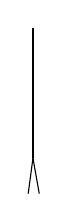
\begin{tikzpicture}[x=1cm,y=1cm]
\draw (0,0) -- (0,-1.65);
\draw (0,-1.65) -- (-0.06,-2.10);
\draw (0,-1.65) -- (0.08,-2.10);
\end{tikzpicture}}}
a) Pour que $F$ raffine $G$, il f et s que ce soit une sous-figure d'une su\deleted{\unsure{f}}bdivision $G'$ de $F$
\[
 :\qquad F\leq G'\preceq G
\]

\deleted{b) Pour que $F$ soit une subdivision de $G$ il f et s. que ce soit un raffinement, et qu'il soit maximal comme}

\deleted{Ainsi, \unsure{dans|dès|donc} $F$}

\uline{Dém}. C'est \unsure{évid\(^{\mathrm{mt}}\)} suffisant, \unsure{Inversemt|Invers\(^{\mathrm{mt}}\)|Inversement}, Supposons $F\ll G$, pour trouver $G'$, on prend $G'=G$ si $F$ est déjà une subd. i.e. $|F|=|G|$. \deleted{\unsure{Sinon}}, Dans le cas général, Soit
\[
\begin{aligned}
 G'&=\bigl\{A\in\unsure{\mathfrak P|\mathscr P|\mathbb P}(L)\mid A\in F\text{ ou }A=\deleted{\unsure{g}}\{x\},\text{ \unsure{avec|où} }x\in |F|\unsure{{}_{K}|\}}\\
   &=F\coprod_{x\in |F|\setminus |G|}\{\{x\}\}
\end{aligned}
\]

\scanpage{27}\mspage{26}
% @ top, cancelled line
\deleted{\unsure{Alors|Ainsi} $F$}

% @ top, paragraph lines 1–4
Ainsi, les relations d'ordre $\ll$ et $\preceq$ de, $F$ se déterminent mutuellement, en termes de $\leq$. Peut-on de $=$ exprimer $\leq$ en termes de $\ll$ et de $\preceq$~?
\margin{??}

% @ upper middle, heading and implication
\uline{NB} On a
\[
 F\leq G\text{ et }F\preceq G\quad\Longrightarrow\quad F=G
\]

% @ middle, argument lines 1–6
\unsure{Il} faudra que ceci soit vrai dans \deleted{\uline{\unsure{toute}}} contrée -- via la condition que si $F\leq G$, $F\ne G$, $\exists\,H$ \inserted{\unsure{figure|fig.}} \uline{non vide} $H$ disjointe de $F$, $H\ll G$ (et si on avait $F\preceq G$, $H$ serait disjointe de $G$ par C5, donc \unsure{on|OK} est ramené à ceci. \deleted{$H\ll G$,}
\[
 H\ll G,\quad
 \underset{\inserted{\substack{\text{(i.e. }H\text{ comp. à }G\text{ et}\\H\cap G=\phi}}}{H\text{ disjointe de }G}
 \quad\Longrightarrow\quad H=\phi_{F}
\]

% @ lower middle, proof lines 1–3; cancelled note above its first line
En effet, $H\leq G'\preceq G$, \deleted{\unsure{$i.e.$ $R_G(H)$|$i.e.$ $R_G'(H)$|$i.e.$ $R_G\lvert H\rvert$}} et $H$ disjointe de $G$ signifie $H$ disjointe de $G'$ \inserted{par \unsure{C1|C5|C4}}, donc $H=\phi$ OK~!)

% @ lower middle, cancelled heading
\deleted{\uline{Famille \unsure{intersection|intersections}}}

% @ lower part, question lines 1–2
Qu'en est-il des autres axiomes des contrées~:

% @ foot, C5
\uline{C5} Si $F\preceq G$, $H$, alors $H$ dis. de $F$ ssi disj. de $G$ trivial, car $|F|=|G|$ et disjonction de $H$ avec $H'$ se voit sur les supports \unsure{par|$\vdash$} $|H|\cap|H'|=\phi$

% @ foot, C6; first capital overwritten
\uline{C6} \deleted{\unsure{R|B|S}}Subdivision induite, on la verra tantôt

% @ foot, C7
\uline{C7} Ext. d'une subd. OK on le vérifiera \unsure{topologique|topologiquement|de tte façon}.

% @ bottom edge, short line; main glyph and following small low circle uncertain
\uline{C}$\unsure{2_0|8_0|\phi_0}$ trivial

\scanpage{28}\mspage{27}
% The opening sentence is outside the four long cancellation strokes.
\deleted{\uline{Proposition}} Soient $F,G$ deux figures ens. de $\mathcal L$. \deleted{\deleted{\unsure{Cons|Con}} Soit \deleted{$\unsure{K|H}$}}
\[
 \deleted{K\deleted{I}=\{(A,B)\in F\times G\mid A^\circ\cap B^\circ\ne\phi\}}
\]
\deleted{de sorte que}
\[
 \deleted{|F\unsure{\mid\cap\mid|\cap\,\mid}G|=\coprod_{(A,B)\in \deleted{I}K} A^\circ\cap B^\circ}
\]
\deleted{et que les \deleted{relations} $A^\circ\cap B^\circ$ $((A,B)\in K)$ forment les classes de la rel. d'équiv. sur $|F|\cap|G|$ borne sup des relations \inserted{d'équiv} \deleted{\unsure{H}}\unsure{induites|induite} par $\unsure{\mathcal R|\mathscr R}_F$ et $\mathcal R_G$. Considérons \deleted{la famille} \deleted{\unsure{des|de}} pour $k=(A,B)$}
\[
 \deleted{\deleted{\unsure{A_k}}\unsure{.}\,C_k=A\cap B}
\]

\diagram{\begin{tikzcd}[ampersand replacement=\&,column sep=small]
 \&\mathcal L\& {}\\
 S\arrow[ur,phantom,"\rotatebox{43}{$\subset$}" description]
  \arrow[d,"{\varphi\ \text{surj}}" ]\& {}\&
 \deleted{\unsure{T}}S'_{\deleted{\unsure{k|n}}}
  \arrow[ul,phantom,"\rotatebox{-42}{$\supset$}" description]
  \arrow[d,"{\varphi'\ \text{surj}}"]\\
 I\& {}\& I'\& {I,\ J\ \text{ens. ord.}}
\end{tikzcd}}

Considérons
\unsure{\diagram{\begin{tikzcd}[ampersand replacement=\&,row sep=small,column sep=small]
 {} \& {} \& S\arrow[dr,hook]\arrow[dddl,<->,"\varphi"{swap,near start}] \& {}\\
 S\cap T\arrow[urr,hook]\arrow[drr,hook]\arrow[ddd,dash,"\psi"'] \& {} \& {} \& L\\
 {} \& {} \& T\arrow[ur,hook]\arrow[dd,"\varphi'"] \& {}\\
 {} \& I \& {} \& {}\\
 \deleted{J}K\arrow[ur]\arrow[rr] \& {} \& I' \& {}
\end{tikzcd}}|\diagram{\begin{tikzcd}[ampersand replacement=\&,row sep=small,column sep=small]
 {} \& {} \& S\arrow[dr,hook]\arrow[dddl,"\varphi"{swap,near start}] \& {}\\
 S\cap T\arrow[urr,hook]\arrow[drr,hook]\arrow[ddd,dash,"\psi"'] \& {} \& {} \& L\\
 {} \& {} \& T\arrow[ur,hook]\arrow[dd,"\varphi'"] \& {}\\
 {} \& I \& {} \& {}\\
 \deleted{J}K\arrow[ur]\arrow[rr] \& {} \& I' \& {}
\end{tikzcd}}}
\unsure{avec}
\[
 K=\operatorname{Im}\bigl(S\cap T\xrightarrow{(\varphi,\varphi')} I\times J\bigr)
 =\bigl\{(i,j')\in I\times I'\mid A_i^\circ\cap \deleted{\unsure{B}}\unsure{A_{i'}^{\prime\circ}|B_{j'}^{\prime\circ}}\ne\phi\bigr\}
\]
si $j=(i,i')$, on aura $\boxed{A_j=A_i\cap A'_{i'}}$
\unsure{et|où} on pose
\[
 \begin{aligned}
 A_i'&=\varphi^{-1}(I_{\leq i})\\
 \unsure{\deleted{\unsure{A}}B_j'|\deleted{\unsure{B}}A_j'}&=\varphi^{\prime-1}(I'_{\leq j})
 \end{aligned}
\]

\scanpage{29}\mspage{28}

\deleted{\unsure{Alors}}

Ainsi

\uline{Proposition} On a construit un Inf de $F$ et $G$ pour $\ll$, on l'appelle la ``figure intersection'' $F.G$.

Attention, ce \uline{n'est pas} \inserted{en général} la figure $F\cap G$, \deleted{\unsure{quand|inter.|intersection}} en se rappelant $F,\deleted{F}G\subset\unsure{\mathfrak P|\mathscr P|\mathbb P}(\unsure{L,|L_1|L})$, \deleted{$G\subset\mathfrak P(L)$}

Nous n'allons considérer cette $F\cap G$ que dans le cas où $F$ et $G$ compatibles, mais alors les deux coïncident~!

Donc la bonne notion d'intersection est le $F.G$. En fait, ça marche pour une famille quelconque de figures, et
\[
 \left|\bigwedge_{i\in I} F_i\right|=\bigcap_{i\in I}|F_i|\quad .
\]

Cette propriété d'existence d'un Inf pour la relation $\ll$ \unsure{l'apparente|s'apparente} \deleted{\unsure{la propriété|la présentation}} à une propriété de ``\uline{modération}''.

\deleted{\uline{Propriété} Si $F'\preceq F$ \deleted{\unsure{, et des}}, alors $F'.G\preceq F.G$ (Immédiat sur supports)~: Subdivision \uline{induite} sur un raffinement.}

\scanpage{30}\mspage{29}
% @ top, proposition heading
\uline{Proposition} Soient $F',F,G$ trois figures.
% @ top, three implications
\[
\begin{aligned}
 \text{a)}\quad F'\ll F&\Longrightarrow F'.G\ll F.G\\
 \text{b)}\quad F'\preceq F&\Longrightarrow F'.G\preceq F.G\\
 \text{c)}\quad F'\leq F&\Longrightarrow F'.G\leq F.G\quad{}^{*}
\end{aligned}
\]
% @ upper right, beside a
\margin{(trivial par déf. de $\ll$ comme Inf)}
% @ upper right, beside b
\margin{(\unsure{résulte} de a), en regardant supports)}
% @ upper left, starred gloss
\margin{$*$ \uline{\unsure{explicitation|explication}}}
% @ upper part, starred formula
\[
 F'.G=\{A\in F.G\mid A\subset |F'|\}
\]

% @ upper part, proof lines 1–2
Prouvons c. Il faut prouver que \deleted{$F'.G$} $F'.G\subset F.G$, et est fermé dans $F.G$.

% @ middle, proof lines 1–5
\deleted{\unsure{or|ces|ce}} Or $F'.G$ est formé des $A\cap B$ $(A\in F',B\in G)$ tels que $A^\circ\cap B^\circ\ne\phi$, et $F.G$ des $A\cap B$ $(A\in F,B\in \unsure{G|L})$ tels que $A^\circ\cap B^\circ\ne\phi$, et dans les deux cas \unsure{le|les} sens de $A^\circ$ (p.r. à $F$, \unsure{dans|ds} $F'$) est le $=$, donc $F'.G\subset F.G$. Prouvons que c'est fermé i.e.
% @ centre, first membership and annotations
Si \deleted{$(\deleted{A\cap B}\qquad A,A'\in F',$}
\[
 \underset{\substack{\rotatebox{-90}{$\in$}\\ F'}}{A}\cap
 \underset{\substack{\rotatebox{-90}{$\in$}\\ G}}{B}\in F'.G\qquad
 \text{i.e. } A^\circ\cap B^\circ\ne\phi
\]
% @ centre, second membership and annotations
\figure{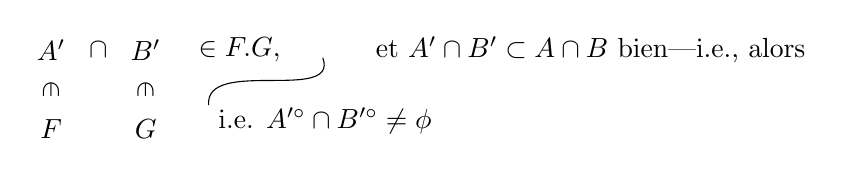
\begin{tikzpicture}[x=1cm,y=1cm]
\node at (0,0) {$A'$};
\node at (.6,0) {$\cap$};
\node at (1.2,0) {$B'$};
\node[anchor=west] at (1.75,0) {$\in F.G,$};
\node[rotate=-90] at (0,-.5) {$\in$};
\node[rotate=-90] at (1.2,-.5) {$\in$};
\node at (0,-1) {$F$};
\node at (1.2,-1) {$G$};
\node[anchor=west] at (4,0) {et $A'\cap B'\subset A\cap B$ \deleted{\unsure{bien|i.e.}}, alors};
\node[anchor=west] (ins) at (2,-.9) {\inserted{i.e. $A'^\circ\cap B'^\circ\ne\phi$}};
\draw (3.45,-.1) to[out=-70,in=95] (2,-.7);
\end{tikzpicture}}
% @ middle lower, conclusion lines 1–4
$A'\cap B'\in F'.G$ i.e. $A'\in F'$. Or on sait que (d'après la théorie de $F.G$) que $A'\cap B'\subset A\cap B\Longrightarrow A'\subset A$, $B'\subset B$, d'où $A'\in F'$ puisque $F'$ fermé dans $F$.

% @ lower left, oblique explanation
% slanted; source note rotated -45 degrees for inspection; final short label below the inverse-image line
\margin{\uline{Expliciter}~: soit
\diagram{\begin{tikzcd}[ampersand replacement=\&,column sep=small,row sep=small]
 G\arrow[r,phantom,"\leq" description]\&F\arrow[d,phantom,"\rotatebox{90}{$\unsure{\preceq|\ll}$}" description]\\
 {}\&F'
\end{tikzcd}}, d'où $G'$ \unsure{avec} $G'\preceq G$, $G'\leq F'$. Alors on a $G'=\{A'\in F'\mid A'\subset |G|\}=\varphi^{-1}(G)$, où $\varphi:F'\to F\ldots$ \unsure{$C_3$.|Cor.|C6.}}
% @ lower right, note on uniqueness; two separate vertical grouping strokes on its left are reproduced
\margin{\figure{\begin{tikzpicture}
\node[anchor=north west,inner sep=0pt,text width=2.05cm] (uppernote) at (0,0) {Un peu vif, on trouve par $F'.G=G'$ un $G'$ tel que
\diagram{\begin{tikzcd}[ampersand replacement=\&,column sep=small,row sep=small]
 F'\arrow[r,phantom,"\preceq" description] \arrow[d,phantom,"\rotatebox{90}{$\leq$}" description]\& F\arrow[d,phantom,"\rotatebox{90}{$\leq$}" description]\\
 G'\arrow[r,phantom,"\preceq" description]\& G
\end{tikzcd}}
mais il faut vérifier encore l'\uline{unicité}};
\draw ([xshift=-4pt]uppernote.north west) -- ([xshift=-4pt,yshift=1pt]uppernote.south west);
\draw ([xshift=-1pt,yshift=-7pt]uppernote.north west) -- ([xshift=-1pt,yshift=-1pt]uppernote.south west);
\end{tikzpicture}}}
% @ lower right, second note; left boundary steps right after the first b line, then descends alongside its continuation
\margin{\figure{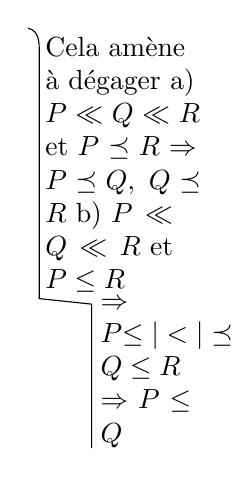
\begin{tikzpicture}
\node[anchor=north west,inner sep=0pt,text width=2.05cm] (lowernote) at (0,0) {Cela amène à dégager a) $P\ll Q\ll R$ et $P\preceq R\Rightarrow P\preceq Q,\ Q\preceq R$ b) $P\ll Q\ll R$ et $P\leq R$};
\node[anchor=north west,inner sep=0pt,text width=1.35cm] (continuation) at ([xshift=7mm,yshift=-2pt]lowernote.south west) {\deleted{$\Rightarrow P\unsure{\leq|<|\preceq}$} $Q\leq R$\\$\Rightarrow P\leq Q$};
\draw ([xshift=-6pt,yshift=3pt]lowernote.north west) .. controls ([xshift=-2pt,yshift=2pt]lowernote.north west) and ([xshift=-2pt,yshift=-2pt]lowernote.north west) .. ([xshift=-2pt,yshift=-6pt]lowernote.north west) -- ([xshift=-2pt,yshift=-2pt]lowernote.south west) -- ([xshift=-3pt,yshift=-2pt]continuation.north west) -- ([xshift=-3pt]continuation.south west);
\end{tikzpicture}}}
% @ lower part, corollary
\uline{Cor.} L'axiome C6 est valable.

% @ lower part, introduction to C7; small 0 is attached to the 7 in this main line, beside the right-note boundary
Vérifions quand même C7$_0$
% @ lower part, order diagram and existence
\diagram{\begin{tikzcd}[ampersand replacement=\&,column sep=small,row sep=small]
 G\arrow[r,phantom,"\leq" description]\arrow[d,phantom,"\rotatebox{90}{$\preceq$}" description]\&F\& {\exists\ \text{subdivision }F'\text{ de }F\text{ qui}}\\
 G'\& {}\&{\text{induise }G'.}
\end{tikzcd}}
% @ bottom, construction
On prend $F'=G'\cup\deleted{(\unsure{F\setminus G|F.G|F\times G}\unsure{2|?})}(F\setminus G)$ (réunion disjointe)
% @ bottom, verification items
Il faut vérifier a) c'est une figure b) que \deleted{\unsure{raffine}}\inserted{subdivise} $F$ et c) qui induit $G'$ sur $G$.

\scanpage{31}\mspage{30}
% @ top, part a
a) $F'$ est une figure. \deleted{\unsure{i.e.}} Notons que \deleted{$|F'|=$}
% @ top, support with braces
\[
 |F'|=\underbrace{|G'|}_{|G|}\cup\underbrace{|F\setminus G|}_{\supset |F|\setminus |G|}\deleted{\unsure{\supset|=}}\supset |F|
\]
% @ upper part, connector
donc, comme $|F'|\subset |F|$, on a
% @ upper part, support equality
\[
 |F'|\unsure{=|\supseteq}|F|
\]
% @ upper part, argument
Il faut prouver que $\forall x\in |F'|=|F|$, $\exists$ plus petit \unsure{élémt|élém\textsuperscript{t}|élément|élt} de $F'$ qui le contienne. Distinguons deux cas

% @ upper middle, first case
1$^\circ$) $x\in |G|=|G'|$, soit $A\in G'\deleted{\unsure{\circ}}$ tel que $x\in A^{\circ(G')\deleted{\unsure{)|?}}}$. Si $B\in F'$ et \deleted{$\unsure{B\supset|B}$} $x\in B$, prouvons $A\subset B$. Si $B\in G'$, c'est évident. Si $B\in F\setminus G$, alors \deleted{$B$ \unsure{contient}} $A^{\circ(G')}\cap B\ne\phi$ donc $A^{\unsure{\circ|\bullet|*}}\subset B$ OK

% @ middle, second case
2$^\circ$) $x\in |\deleted{\unsure{G}}F|\setminus |G|$, alors les $\deleted{\unsure{B}}A\in F'$ qui contiennent $x$ ne sont pas dans $G'$, ils sont donc dans $F\setminus G$. D'autre part, l'unique \unsure{élémt|élém\textsuperscript{t}|élément|élt} $A$ de $F$ tel que $x\in A^{\circ(F)}$ n'est pas dans $G$ puisque $x\notin |G|$, il est donc dans $F\setminus G$, et \deleted{\unsure{si $x\in A$}} c'est lui plus petit él. de $F$ et à fortiori de $F\setminus G$) qui contient $x$, OK~!

% @ lower middle, part b
b) $F'$ \deleted{\unsure{raffine}}\inserted{subdivise} $F$. Comme $|F'|=|F|$, il faut voir \unsure{seult|seulement} que $F'$ raffine $F$. Donc \deleted{que \unsure{tout}} que
% @ lower part, cancelled attempt
\deleted{1$^\circ$) \deleted{$\forall$} $A\in F'$, \unsure{et} \inserted{l'ens $F^A$ des $B\in F$ tels que $A\subset B$} \unsure{est contenu dans|contienne} un plus petit}
% @ one continuous source cancellation; wrappers split only to place the cancelled insertion in the margin
\margin{\deleted{\inserted{\unsure{a un plus petit|$=$ un plus petit}}}}
\deleted{\unsure{élémt|élém\textsuperscript{t}|élément|élt} de $F$. C'est \unsure{évident} si $A\in F$ c'est \unsure{évident}. Si}
\deleted{\unsure{str.} de de $F'$ \unsure{raffine} $F$. Si}

% @ lower part, restated first condition
1$^\circ$) \deleted{$\forall$} $A\in F'$, l'ens $F^A=\{B\in F\mid \deleted{\unsure{B}}A\subset B\}$ a un plus petit \unsure{élémt|élém|élément|élt}. C'est évident si $A\in F$ \deleted{$(B=A)$} (on prend $B=A$) et si $A\in G'$, c'est vrai puisque $G'\ll F$.

% @ bottom, second condition
2$^\circ$) Si $A\in F'$, $B\in F$, alors $A\cap B$ est \deleted{\unsure{$\mathcal R_{F'}$-satu.|$\mathscr R_{F'}$-satu.|$Q_{F'}$-satu.|$\mathcal O_{F'}$-satu.}}\inserted{fermé dans $F'$}, i.e. réunion \unsure{de|des} strates de $F'$. Si $A\in G'$, comme $G'\ll F$, $A\cap B$ est réunion de strates de $G'$, qui sont aussi des strates de $F'$.

\scanpage{32}\mspage{31}

Si $A\in F\setminus G$, $A\cap B$ est réunion de strates de $F$. \deleted{\unsure{Reste}} reste \unsure{à|:} voir que une strate \inserted{\unsure{$G$|$\in$|e}} de $F$ est réunion de strates de $F'$. Soit $A$ cette strate de $F$. \deleted{\unsure{On|les|le}}
\[
 \deleted{A=\bigcup_{\substack{B\in F\\B\leq F}}B^\circ}
\]
Si $A\notin G'$, \unsure{donc|alors} $A\in F\setminus G'\subset F'$, et on gagne. Si $A\in G$, alors (comme $G'\preceq G$) $A$ est réunion de strates de $G'$, qui sont des strates de $F'$, et on gagne encore.

% slanted
\margin{Ultra faux}
\uline{Corollaire} Le \deleted{raffinement}\inserted{subdivision} précédente $F'$ de $F$ est caractérisée par \inserted{chacune} des \unsure{pr.|pro.} propriétés équivalentes suivantes~:

\deleted{a) Pour toute subdivision $F''$ de $F$ qui induit $G'$ sur $G$, on a $F''\preceq F'$ -- i.e. $F'$ est \deleted{\uline{maximal}}\inserted{un plus grand \unsure{élémt|élément|élt}}, pour $\preceq^{*}$, \unsure{dans|pour} l'ens des subdivisions de $F$ qui induisent $G'$ sur $G$.}
% slanted
\margin{$*$ ou pour $\ll$, cela revient au $=$ parmi des subdivisions d'une $=$ $F$}
% slanted; live state preferred, whole-note cancellation explicitly retained as an alternative.
\margin{\unsure{\figure{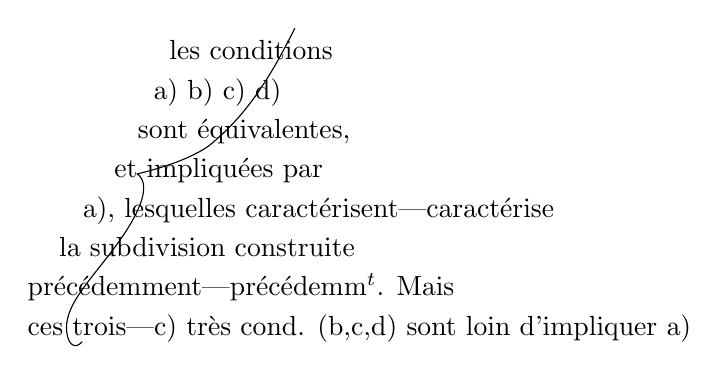
\begin{tikzpicture}[x=1mm,y=1mm,
 every node/.style={anchor=base west,inner sep=0pt}]
 \node at (18,0) {les conditions};
 \node at (16,-5) {\deleted{\unsure{a)}} b) c) d)};
 \node at (14,-10) {sont équivalentes,};
 \node at (11,-15) {\unsure{et} \uline{impliquées} par};
 \node at (7,-20) {a), lesquelles \unsure{caractérisent|caractérise}};
 \node at (4,-25) {la subdivision construite};
 \node at (0,-30) {\unsure{précédemment|précédemm$^{t}$}. Mais};
 \node at (0,-35) {\unsure{ces trois|c) très} \unsure{cond.} (b,c,d) \unsure{sont} \unsure{loin} d'impliquer a)};
 \draw (34,4)
  .. controls (31,-2) and (28,-7) .. (23,-11)
  .. controls (20,-13) and (16,-14) .. (14,-14.5)
  .. controls (16,-16) and (14,-20) .. (11,-24)
  .. controls (8,-28) and (5,-31) .. (5,-34)
  .. controls (5,-36) and (6,-37) .. (7,-35.8);
\end{tikzpicture}}|\deleted{les conditions \deleted{\unsure{a)}} b) c) d) sont équivalentes, \unsure{et} \uline{impliquées} par a), lesquelles \unsure{caractérisent|caractérise} la subdivision construite \unsure{précédemment|précédemm$^{t}$}. Mais \unsure{ces trois|c) très} \unsure{cond.} (b,c,d) \unsure{sont} \unsure{loin} d'impliquer a)}}}

% Small additional a)-like label above the end of application, attachment uncertain.
b) L'application \inserted{\unsure{a)}} can. associée à $F'\preceq F$
\[
 \varphi:F'\longrightarrow F
\]
induit une bijection
\[
 F'\setminus G'\xrightarrow{\sim}F\setminus G.
\]
\margin{\figure{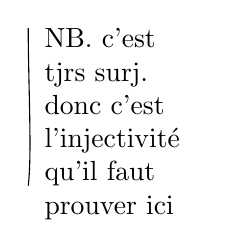
\begin{tikzpicture}[x=1mm,y=1mm]
 \draw (0,0) .. controls (0,-7) and (0.5,-16) .. (0,-20);
 \node[anchor=north west,inner sep=0pt,align=left,text width=20mm] at (2,0) {NB. c'est tjrs surj. donc c'est l'\uline{injectivité} qu'il faut prouver ici};
\end{tikzpicture}}}

c) \deleted{Les strates ouvertes de $F'$ qui ne \unsure{sont}} \inserted{$\forall A\in F\setminus G$, $A^\circ$ est une \unsure{str.te|strate|str.} ouverte} de $F'$.

d) $F'\supset F\setminus G$, i.e. $\forall A\in F\setminus G$, on a $A\in F'$.

\uline{Dém} On va prouver p. ex
\[
 \text{d)}\Longrightarrow\text{b)}\Longrightarrow\text{c)}\Longrightarrow\text{a)}\Longrightarrow\text{d)}
\]
\deleted{\uline{\unsure{Dém}}} $\text{d)}\Rightarrow\text{b)}$ Si $(F\setminus G)\subset F'$, alors $\varphi\mid F\setminus G$ est l'\deleted{\unsure{identité}}inclusion \deleted{(trivial)} \inserted{can. $F\setminus G\hookrightarrow F$}, \deleted{donc} donc il reste à prouver
\[
 F\setminus G=F'\setminus G'.
\]

\scanpage{33}\mspage{32.}
% @ top, 1°)
\deleted{\unsure{R|P|Or}} $\Rightarrow$ 1°) $F\setminus G\subset F'\setminus G'$ i.e. Tout $A\in F\setminus G$ est $\notin G'$. En effet, si on avait $A\in G'$, on aurait $|A|\subset|G'|=|G|$ donc \deleted{$A\in$} (comme $G\leq F$) $A\in G$.

% @ left edge, along 1°), 2°), and the following proof
% margin note written sideways; long separator rule to its right
% Approximate bowed separator geometry; source crop box [65,125,285,1755].
\margin{\figure{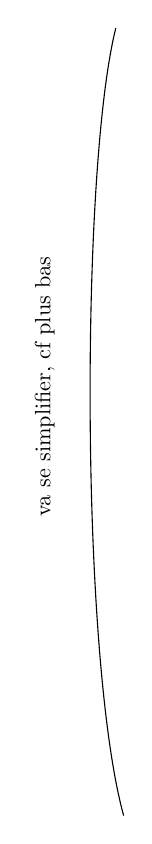
\begin{tikzpicture}[x=1cm,y=1cm]
\draw[line width=.4pt] (1.0,0) .. controls (.45,2.0) and (.45,8.2) .. (.90,10);
\node[rotate=90,anchor=west,scale=.8] at (0,3.7) {va se simplifier, cf plus bas};
\end{tikzpicture}}}

% @ upper middle, 2°)
2°) $F'\setminus G'\subset F\setminus G$ Soit $A'\in F'\setminus G'$, prouvons $A'\in F\setminus G$, et d'abord $A'\in F$. \deleted{\unsure{On a}} Soit $A$ le plus petit él. de $F^{A'}$ donc $\underline{\rule[-.15ex]{.35pt}{.55ex}\,A'\unsure{\subset|\in|\subseteq} A^{\unsure{\deleted{\unsure{\prime|\ast|?}}|\varphi|q}},\ A'^{\circ(F')}\subset A^{\unsure{\deleted{\unsure{\prime|\ast|?}}|\varphi|q}\circ(\unsure{F}}\,\rule[-.15ex]{.35pt}{.55ex}}$ prouvons que $A'=A$ (d'où $A\in F$). \deleted{\unsure{On a|Or}}

% @ middle, Je dis
Je dis que $A\in F\setminus G$ i.e. $A\notin G$, sinon on aurait $A\subset|G|=|G'|$ donc $A'\in G'$ puisque $A'\in F'$ et $G'\leq F'$, absurde. \deleted{Mais} Donc $A\in F\setminus G$, donc $A\in F'$, \deleted{et} Il en résulte que $A^{\circ(F)}=A^{\circ(F')}$ (car $F'\preceq F$\inserted{il suffirait $F'\ll F$}\deleted{)} cf lemme plus bas) et \unsure{\uline{bien}|\deleted{bien}} \deleted{$\unsure{F|\in|E}$} $A,A'\in F'$ tels que $A'^{\circ(F')}\subset A^{\circ(F')}$, ce qui prouve $A=A'$.

% @ lower middle, Donc
Donc \unsure{on a} prouvé que $\deleted{\unsure{F|A}}A'\in F'\setminus G'\Rightarrow A'\in F$. Prouvons qu'on a $A'\notin G$ (d'où $A'\in F\setminus G$\deleted{)}, qed). \unsure{Sinon|Si} on aurait $A'\in G$, on aurait $A'\subset |G|=|G'|$, d'où (comme $A'\in F'$ et $G'\leq F'$) $A'\in G'$, absurde.

% @ lower third, cancelled b) to c)
\deleted{b) $\Rightarrow$ c) \inserted{On suppose b) i.e. $\varphi$ induit $F'\setminus G'\overset{\sim}{\longrightarrow}F\setminus G$} Soit $A\in F\setminus G$, prouvons que $A^{\circ(F)}$ est un \uline{\unsure{str.$^{t}$-ouvert|str.t-ouvert|strate ouverte} pour \deleted{$\unsure{F|A|la}$} $F'$}. Soit $A'\in F'\setminus G'$ l'unique élément \deleted{de} tel que $\varphi(A')=A$.}
% The oblique cancelling strokes end above this final line; state remains open.
\unsure{Prouvons $A'^{\circ(F')}=A^{\circ(F)}$.|\deleted{Prouvons $A'^{\circ(F')}=A^{\circ(F)}$.}}

% @ bottom, b to c
b $\Longleftrightarrow$ c \deleted{\unsure{Posons}} On a $|F|\setminus|G|=|F'|\setminus|G'|$, soit $U$, Posons $F\setminus G=I^{\unsure{\ast|k|+|\leftarrow}},\ F'\deleted{\unsure{\times|\setminus}}\unsure{\setminus}G'=I'^{\unsure{\ast|k|+|\leftarrow}}$ (parties ouvertes des ens d'indices ordonnés $I$, \deleted{$\unsure{A|\Delta}$} $(=\unsure{F|P})$, $I'(=F')$. On a
